\begin{center}
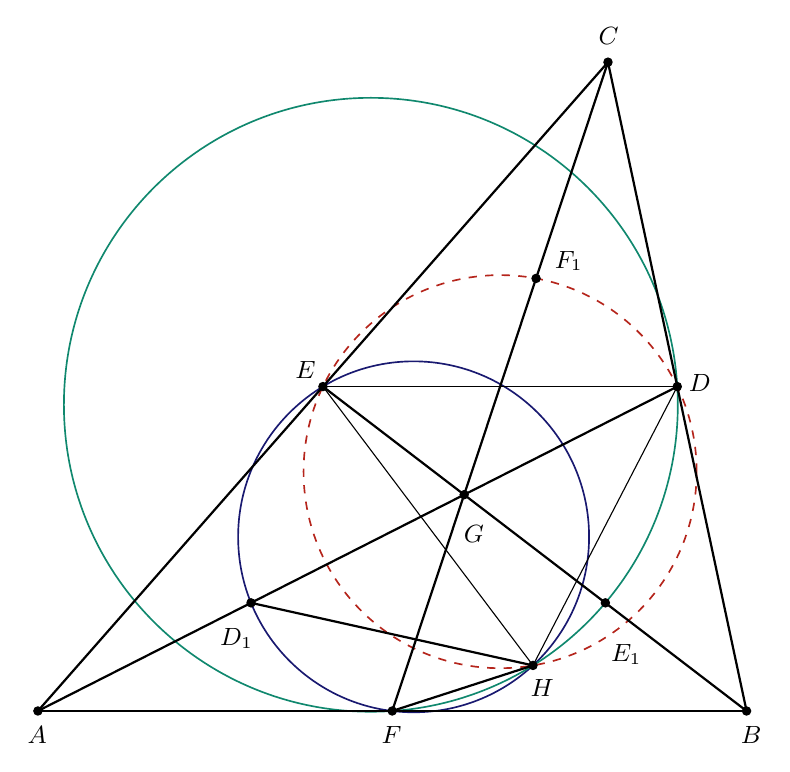
\begin{tikzpicture}[scale=1, font=\small]
    \coordinate (A) at (0, 0);
    \path (A) ++(-0.008, -0.3) node[inner sep=0pt] {$A$};
    \coordinate (B) at (9, 0);
    \path (B) ++(0.06, -0.303) node[inner sep=0pt] {$B$};
    \coordinate (C) at (7.24, 8.24);
    \path (C) ++(0.008, 0.33) node[inner sep=0pt] {$C$};
    \coordinate (D) at (8.12, 4.12);
    \path (D) ++(0.287, 0.04) node[inner sep=0pt] {$D$};
    \coordinate (E) at (3.62, 4.12);
    \path (E) ++(-0.223, 0.215) node[inner sep=0pt] {$E$};
    \coordinate (F) at (4.5, 0);
    \path (F) ++(-0.009, -0.3) node[inner sep=0pt] {$F$};
    \coordinate (G) at (5.41333, 2.74667);
    \path (G) ++(0.123, -0.495) node[inner sep=0pt] {$G$};
    \coordinate (D1) at (2.70667, 1.37333);
    \path (D1) ++(-0.184, -0.454) node[inner sep=0pt] {$D_{1}$};
    \coordinate (E1) at (7.20667, 1.37333);
    \path (E1) ++(0.266, -0.658) node[inner sep=0pt] {$E_{1}$};
    \coordinate (F1) at (6.32667, 5.49333);
    \path (F1) ++(0.415, 0.221) node[inner sep=0pt] {$F_{1}$};
    \coordinate (H) at (6.28748, 0.5786);
    \path (H) ++(0.116, -0.287) node[inner sep=0pt] {$H$};

    \draw[semithick, MidnightBlue] (4.77139, 2.21195) circle (2.22853);
    \draw[semithick, PineGreen] (4.22861, 3.8888) circle (3.89825);
    \draw[semithick, BrickRed, dashed] (5.87, 3.03945) circle (2.49601);
    \draw[thick] (A)--(B);
    \draw[thick] (B)--(C);
    \draw[thick] (C)--(A);
    \draw[thick] (A)--(D);
    \draw[thick] (B)--(E);
    \draw[thick] (C)--(F);
    \draw[thin] (D)--(E);
    \draw[thin] (E)--(H);
    \draw[thin] (H)--(D);
    \draw[thick] (D1)--(H);
    \draw[thick] (H)--(F);

    % Radius cetak titik tetap 1.5pt saat scale diubah.
    \pgfgettransformentries{\studioXX}{\studioYX}{\studioXY}{\studioYY}{\studioDX}{\studioDY}
    \pgfmathsetlengthmacro{\studioRadiusTitik}{1.5pt/veclen(\studioXX,\studioYX)}
    \foreach \s in {A,B,C,D,E,F,G,D1,E1,F1,H}
        \filldraw (\s) circle (\studioRadiusTitik);
\end{tikzpicture}
\end{center}
